\cleardoublepage
\chapter{Systematic Review}

\section{Introduction}
This chapter reviews statistical and neural network algorithms for the automatic classification of melanoma. Following a discussion on the effectiveness of techniques and whether they are useful within clinical environments. 

%Start with a broader scope and mention the classification of lesions with NN techniques, explainability, etc.

\section{Skin Lesions}

\section{Diagnostic Procedures}

\section{CAD Systems for Skin Lesion Diagnosis}

\section{Case-Based Reasoning}

\section{Discussion}
%Mention a wide range of techniques espeically around NN techniques and hybrid models, feature detectors, direct classification (CNN, DNN, etc)

Melanoma is a deadly skin cancer that frequently results in the death of patients if develops into metastatic melanoma. This refers to when the cancer has burrowed past the skin and makes its way into blood and internal organs. From this point is it far more difficult to remove.

Melanoma develops from melanocyte cells, which in turn produce melanin resulting in skin pigmentation (brown patch of skin). This means there are visual characteristic of melanoma as it continues to grow. Alongside the necessity to improve the diagnostic accuracy the visual characteristics being ideal for the development of computer vision-based algorithms, this has sparked the creation of algorithms and in turn papers.

When doctors utilize a clinical diagnostic tool they should be capable of rationalising and building explanations based on the data provided from that tool. Currently, many techniques\cite{Andre2017} called named `black box' approaches produce parallel diagnosis that lacks adequate explanations for clinical environments. These provide insufficient information for use within some clinical environments\cite{Andre2017}. Instead, it would be beneficial for doctors to follow procedures they are familiar with, such as diagnostic procedures including ABCD rules. The reviewed techniques aim to automate the ABCD rules using various statistical and machine-learning techniques. Many are interpretable and suitable for clinical environments.

Hybrid machine learning techniques are recently gaining traction, an example by Ali combines results from both Gaussian naive Bayes (GNB) and a CNN\cite{Ali2020b} for border irregularity detection. The CNN ensures high-accuracy classification by finding the relationship between each component, and the GNB is interpretable. Results are combined using an ensemble approach, making a prediction probability. Such techniques are promising for use within clinical environments.

There is a lack of literature describing adequate visual representations for doctors, and it is understandable as there is still little evidence proving that CAD systems improve doctors decision making-processes\cite{FerrantediRuffano2018}. It would be beneficial to create literature describing a catalogue of different visualisations that benefit doctors. Putting all this information together, alongside a questionnaire, might provide further insight into the visualisations that might be most useful to doctors.

%Supporting algorithms such as deepshap

\section{Research Methodology}
The reason for writing this review was to select the best approaches to skin cancer detection and regarding whether they can be utilised within clinical environments. 

Combining the information helps specify what is currently known in literature and highlighting what areas need further work.

Literature is chosen considering techniques that are explainable or have supporting techniques developed for explainability.

\subsection{Research Questions}
The goal of this systematic review is to answer the following questions:

\begin{enumerate}
	\item What are the major techniques developed for the detection of skin cancer?
	\item Are these techniques suitable for use within clinical environments?
	\item Can these techniques be supported with other algorithms to improve explainability?
\end{enumerate}

\subsection{Search Criteria}

\begin{table}
	\begin{tabular}{}
	\hline
	Search Term & Set of Key Words \\
	\hline
	Skin & skin cancer, skin treatments
	\hline
	\end{tabular}

\end{table}

\section{Artificial Neural Network (ANN) Techniques}
An artificial neural network is a nonlinear statistical prediction technique.

\section{ Convolutional Neural Network (CNN) Techniques}

\section{Deep Neural Network (DNN) Techniques}

\section{Kohonen Self-Organising Neural Network (KNN) Technqiues}

\section{Generative Adveserial Network (GAN) Techniques}


\section{Explainability Techniques}
The techiques mention in this section are ones including deepshap that are used alongside exisiting DNN techniques to make models more explainable.

The Local Interpretable Model-agnostic Explanations (LIME)

LIME has been tested in healthcare for the analysis of breast tumor classification\cite{rafferty2022}, and diagnosis of pigmented skin lesions\cite{duell2021}. Its ability to calculate feature importance for machine learning predictions has made it a valuable tool for improving the interpretability of AI models in the medical domain.

\section{Ensemble Learning Techniques}
Ensamble learning is a branch of machine learning based on the decision-making process to intergrate it into systems better\cite{xu2022}. Decision-making is the process of making a choice among many options and summarizing evidence to draw a conclusion. An example is case-based reasoning which involves classifying and presenting visually or statistically similar cases and their results.

%Mention paper showing improved accuracy of GPs using machine learning algorithms

\section{Hybrid machine learning techniques}
Hybrid machine learning are techniques that aims to use the superior accuracy of deep learning algorithms that are difficult to interpret alongside more explainable algorithms inlcuding bayesian networks, SVMs and others. Results are then combined to reach a result.

\section{Feature Extraction Techniques}
Many CAD frameworks follow a methodology for the classification of skin lesions. These are listed below:

\begin{enumerate}
	
	\item Segmentation – Image segmentation is the process of partitioning an image into multiple segments for more accessible analysis. These areas can be separated manually by a dermatologist (known as the ground truth) or separated automatically using statistical or machine learning algorithms.
	
	\item Feature Extraction - Gathering features through filtering, morphology and other statistical approaches. ABCD rules include asymmetry, border, colour, and dermoscopic structures.

	\item Combination - Combining the extracted features before using Principal Component Analysis (PCA) or after classification using Bayesian Fusion. Others combine the results using the Total Dermoscopy Score (TDS).
	
	\item Classification – Measuring the results from the features and components through classification. Containing the final diagnosis of the type of skin lesion (Naveus, SK, or Melanoma)

\end{enumerate}

\subsection{Segmentation}
Yading Yuan and Yeh Chi Lo describe a fully convolutional network (FCN) with an accuracy of 91.7\% with the PH$^2$ dataset\cite{Yuan2017a}. FCN is a variation of a CNN using 1x1 convolutions instead of dense layers. Essentially, an FCN forms a more complex function (generating a more complex neural network), whereas the CNN forms a less complex function, likely to degrade essential features. Therefore, more data is needed to train an FCN effectively than a CNN. After the convolution layers, transposed convolution layers (or deconvolution) and other layers (un-pooling) up-sample the input feature map to the size of the input image. Then, the network, trained from ground truth (human-generated segmentation mask) and the original images, can automatically generate segmentation masks based on textures and colours of the skin lesion provided. There are dozens of examples of this, such as SegNet\cite{Badrinarayanan2017}, which is another transposed CNN not designed initially for skin lesions but is effective at segmenting skin lesions.

E. Meskini et al. proposed using Otsu binarisation - a threshold technique that is effective at locating the border of a skin lesion after segmenting using Segnet\cite{Meskini2018}. Researchers proposed that when analysing the skin lesion border using ABCD rules, the original SegNet methods were ineffective because the ground truth is subjective - ineffective at finding the border cut-off between the skin lesion and skin. While SegNet has a 91.7\% with the PH$^2$ dataset, the data is not effective at finding the precise border cut-off required for accurate border classification using ABCD rules. Therefore, researchers proposed the Otsu threshold to find the skin lesion border after segmenting using SegNet. Fan proposes another technique that uses a saliency-based segmentation approach to capture the area, followed by an Otsu threshold\cite{Fan2017} to find the border cut-off from the skin lesion with a precision of 96.78\% validated using the PH$^2$ dataset.

Pedro M.M. Pereira et al. proposed local binary pattern clustering (LBPC) to exaggerate the border, producing accurate results when classifying ABCD rules than ground-truth borders in the PH$^2$ dataset\cite{Pereira2020}. Local binary patterns (LBP) are texture descriptors calculated by comparing the centre pixel (of each pixel in the grey scaled image) with the eight neighbouring pixels as 'i', and converting it to a binary using the equation:  [$if centroid > neighbour_i =  0, otherwise = 1$]. These eight neighbouring values produce a binary of 01101100 (decimal of 108) and change the centroid to 108. Next, the described process repeats on each other pixel in the image. Finally, the newly filtered image subtracted from the original grey-scaled image creates a segmentation mask with an accurate border cut-off. Finally, Pereira describes classification methods using SVM or FNN presenting the extracted border with an accuracy of 79\% and 77\% (respectively) with the MED-NODE dataset.

\subsection{Handcrafted Features}
Handcrafted features are the extraction of particular features using statistical algorithms the benefit of separating data into components is a more accessible breakdown, improving explainability. In addition, this might instantiate trust for use within a clinical environment and prove more helpful to doctors.

\subsubsection{Asymmetry}
Asymmetry can be measured using the bi-fold technique, which involves drawing a line down the middle of the skin lesion and comparing the two halves to confirm whether the sides match, on both the horizontal and vertical axes, as shown in \ref{lit-asym}. If the two sides are greatly different, it could be a warning sign of melanoma. Asymmetry can be measured using the shape\cite{Zaqout2016}, colour\cite{Kasmi2016}, and texture\cite{Ali2020a}.

\begin{figure} 
\centering
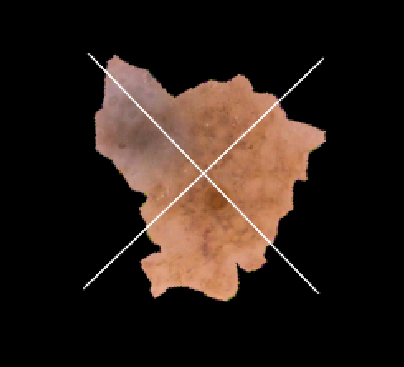
\includegraphics[scale=0.5]{images/asym1.png}
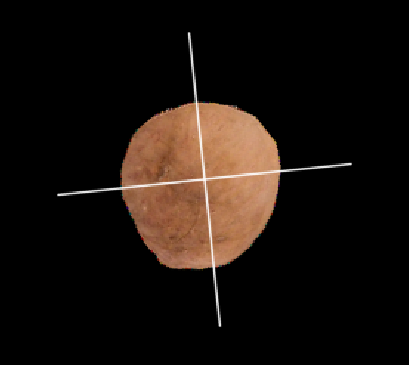
\includegraphics[scale=0.5]{images/asym2.png}
\caption{Images of two skin lesions from the PH$^2$ dataset showing the asymmetry calculated from moments.}
\end{figure} \label{lit-asym}

Measuring the asymmetrical shape requires a precise border cut-off. Ihab S. Zaqout\cite{Zaqout2016} describes a technique using the centroid and rotation of the skin lesion using moments of inertia. By Folding the skin lesion on both vertical and horizontal axes subtracting the opposite half. Pixels that cannot subtract are summed and compared with a threshold considering the skin lesion asymmetrical if the combined sum is more than the threshold.

Reda Kasmi and Karim Mokrani\cite{Kasmi2016} describe creating a grid of 20x20 pixels of the skin lesion image and converting it into the LAB colour space. Next, each block's average colour is compared with a perpendicular block (vertical and horizontal axes) using the three-dimensional Euclidean luminance distance, a-axis, and b-axis. If more than half of the colour comparisons are over the threshold, that axis is considered colour asymmetrical. Blocks that have no symmetrical pair are ignored. Finally, luminance calculated separately prevents brightness problems. This technique has an accuracy of 94\% with a private dataset.

Measuring similarities in texture can be achieved by using SIFT-based similarity and projection profiles\cite{Ali2020a}. SIFT is scale-invariant and helpful for texture components with varying texture quality. First, the skin lesion is split vertically and horizontally across the centre into four halves, comparing texture components on the symmetrical halves and measuring the similarity. Lastly, the projection profile in the x and y directions generates histograms. These results train a decision tree and have an 80\% accuracy of the ISIC 2018 with 204 images privately annotated for ABCD rules and combined.

\subsubsection{Border}
Estimating border irregularities involves splitting the skin lesion into eight equal sections (through the centroid), where each section with tight corners and convexity is considered irregular. Each irregular section of the border adds a score of 1 ranging from 0 to a total of 8, as shown in figure \ref{borders}.

\begin{figure}
\centering
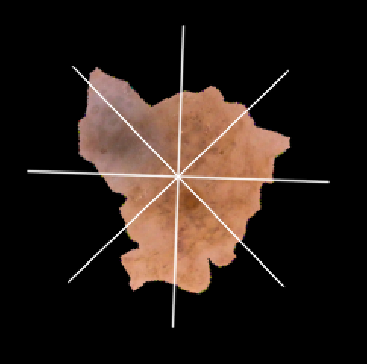
\includegraphics[scale=0.5]{images/bord1.png}
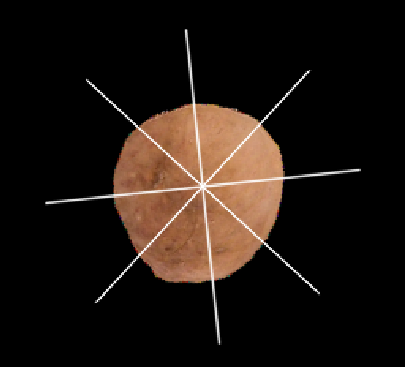
\includegraphics[scale=0.5]{images/bord2.png}
\caption{Images of two skin lesions split into 8 sections using moments, each border is measured for irregularity.}
\end{figure} \label{borders}

Border irregularity contours were found by splitting the skin lesion into eight segments around the centre, and then calculating a fitting error for each. If the error is larger than 0.05 (x contour), that area is considered irregular\cite{Kasmi2016}.

Abder Rahman H. Ali et al. calculate the compactness of each border by first calculating the contour around the area of the lesion containing x and y positions. Next, measure the space between each position to estimate the compactness. The tighter the curves and corners, the more contour positions, revealing irregular borders within a segment, combining all of these scores creates the irregularity index\cite{Zaqout2016}.

Fractal dimensions (FDs) is a statistical index measuring the detail in a pattern changing with the image scale index. One technique called box-counting increases values if there are more corners and edges around the border. The higher the value demonstrates the level of border irregularity. Ali describes using machine learning alongside Zernike moments, and convexity measurements for a high-accuracy border irregularity classification\cite{Ali2020b}. However, results are ambiguous because the output is either ``irregular'' or ``regular'' border (not relating to the TDS). Thus, conforming to the TDS and splitting the border into eight sections would make it more interpretable and useful o doctors. However, a hybrid GNB and CNN approach are combined to allow interpretability through GNB.

\subsubsection{Colour}
Colour refers to the shades of pigment within the area of a skin lesion, not referring to abnormalities relating to bruises, crust, and grazes. Melanoma usually contains more than two colours compared with benign lesions, singular in colour. Skin lesions can consist of one or many colours: white, red, light brown, dark brown, blue-grey and black.

Finding colour variations has been achieved by calculating the normalised standard deviation of the red, green, and blue components\cite{She2007}. The normalisation process improves the recognition of normal skin pigmentation, which would show pigmentation levels, making comparisons easier between different skin lesions.

Arthur Tenenhaus, et al. utilise joint learning using Kohonen map, and k-means clustering\cite{Tenenhaus2010}. Five random pixels create a 5 by 5 Kohonen map represented by 25 neurons in a neural network for each skin lesion in the dataset. Colour variations on a 25-dimensional vector find the proportions of pixels projected onto each of the 25 neurons. Next, K-means classifies the skin lesions set by the number of colours found by dermatologists. Only four colours were present in the dataset in this scenario, while seven could be. Eventually, the colour components are represented as a 42-dimensional vector and are passed into a KL-PLS based classifier to detect variations in colour at 66\% using a private dataset.

Reda Kasmi, et al. locate the number of colour variations by converting the image into the LAB colour space matching the colour ranges that can be perceived by human eyes\cite{Myridis2014a}, measuring the average colour distribution of the dataset and assigning each colour as a threshold range. Next, the Euclidean distance between each colour threshold is compared with each pixel colour\cite{Kasmi2016}, finding the closest matching colour of the six colours. Finally, removing the areas of colour with less than 5\% prevents the classification of dots. This approach uses a colour range of white, light brown and dark brown. However, there is a static threshold value for the other colours, which would be unlikely to cover the ranges of the colours, including red, blue-grey, and black.

\subsubsection{Dermoscopic structures}
Dermoscopic structure refers to structures on the skin lesion, including pigment networks, structureless areas, dots, globules, streaks, white structures, and 22 others (not including sub-types). Variations of pigment networks are more commonly found in melanoma\cite{Anantha04} and are therefore a valuable feature for automatic classification. Similarity other features such as milia-like cysts, a sub-type called milia-like cysts (MLC) called cloudy MLC appears more frequently on melanoma than SK, with a specificity of  99.1\% specificity\cite{Stricklin2011}.

Javier López-Labraca et al.\cite{Lopez-Labraca2018} describes a statistical approach to classifying melanoma using dermoscopic structures through Gabor filtering, support vector machines, and Bayesian fusion. This technique uses a form of soft segmentation to find the area of these dermoscopic features. Firstly the structures are located using Gabor filtering using different values to find fissures and globules. Each structure is then compared with a trained SVM model to check the similarity of the detected features. The results from the model are then combined using Bayesian fusion to reach a result of malignant or benign. Finally, training a CNN model alongside an SVM improves the retractability of dermoscopic structures; compared to a standalone CNN model.

\subsection{Combining ABCD Rules}
This section describes combining features from the ABCD rules into a classification between malignant, suspicious or benign after considering all clinical features. Again, meta-data and texture can potentially improve the results.

Maryam Ramezani et al. proposed a method to extract features from ABCD rules storing them in vectors and extracting the texture as a GLCM. First, these 187 features are shrunk to 13 using PCA\cite{Ramezani2014}. Next, the data trains an SVM to classify skin lesions into benign or malignant with an accuracy of 82.2\% on macroscopic images using a private dataset.

Other methods output TDS\cite{Zaqout2016, Zhang2018}, which combines them using: [(Asymmetry x 1.3) + (Border x 0.1) + (Colour x 0.5) + (Diameter x 0.5)]. A statistical model for each ABCD rule outputs a score in the same format. The benefit is interpretability because it follows the diagnostic procedure. The technique achieved an accuracy of 90\% using a private dataset.

\section{Datasets}

\section{Challenges of Explainability}

\section{Conclusion and Future Work}
Many techniques utilise ABCD rules to produce an automatic and interpretable diagnosis. Interestingly, many focus on detecting and classifying asymmetry, border, and colour (ABC) or dermoscopic structures, but neither combine the whole ABCD rules into a single framework. Despite dermoscopic structures providing a means of diagnosing problematic forms of melanoma, including mimics (seborrhoeic keratosis)\cite{Izikson2002}, and non-pigmented melanomas. Thus, it would be valuable to combine both into a single system for possibly higher accuracy.

Despite various valuable features, asymmetry rarely utilises techniques other than statistical models. For example, researchers highly focused on border irregularity and dermoscopic structures, leading to hybrid machine-learning models for their assessment. However, asymmetry still utilises statistical approaches to measure and combine shape, colour, and texture. It would be beneficial to transform this data and process it using an SVM, improving accuracy.

Utilising external data, including feeling, touch, age, and location on the body, are helpful to doctors when diagnosing skin conditions, but is not mentioned in any of the discussed techniques. It would be beneficial to implement this data into the decision-making process.
